\documentclass[12pt]{article}
\usepackage{setspace}  % To use linespacing
\usepackage{indentfirst} % Indents first line after sections
\usepackage{amssymb} % For \mathbb
\usepackage{enumerate} % For changing labels of enumerate
\usepackage[margin=1in]{geometry} % For editing margins
\usepackage{tikz} % Tikz drawing for graphs
\usetikzlibrary{arrows.meta} % Allows customizing arrows
\usetikzlibrary{backgrounds} % For framing a tikzpicture
\usepackage{amsmath}

% Make new commands
\newcommand{\N}{\mathbb{N}}
\newcommand{\R}{\mathbb{R}}
\newcommand{\Z}{\mathbb{Z}}
\newcommand{\abs}[1]{\left|#1\right|}
\newcommand{\paren}[1]{\left(#1\right)}
\newcommand{\fivespace}{\space\space\space\space\space}

\newcommand{\be}{\begin{enumerate}}
\newcommand{\ee}{\end{enumerate}}
\newcommand{\seti}[1]{\setcounter{enumi}{#1}}
\newcommand{\setii}[1]{\setcounter{enumii}{#1}}

% Start main document
\begin{document}
\onehalfspacing
\hfill Frank Cline

\hfill Math 307

\hfill HW 8

% Sections
% 6.6 # 10, 11, 13
% Additional Problems

% SECTION 6.6
\section*{6.6}
\be

% 10
\seti{9}
\item 
	\be
	% 10 a
	\item Use Kruskal's algorithm to find a minimum spanning tree of the graph below. Label the edges in alphabetical 
	alphabetical order as you choose them. Give the weight of the minimum spanning tree.\\
	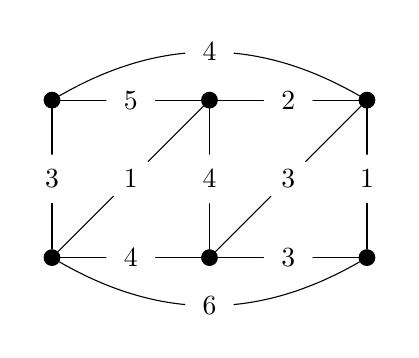
\begin{tikzpicture}
	\begin{scope}[every node/.style={circle,draw, fill= black, inner sep = 2pt}]
	    	\node (1) at (0,0) {};
		\node (2) at (0,2) {};
	    	\node (3) at (2,2) {};
		\node (4) at (4,2) {};
	    	\node (5) at (4,0) {};
	    	\node (6) at (2,0) {};	
	\end{scope}
	
	\begin{scope}[>={Stealth[black]},
	              every node/.style={fill=white,circle},
	              every edge/.style={draw=black}]
		\path (1) edge node{3} (2);
		\path (1) edge node{1} (3);
		\path (1) edge node{4} (6);
		\path (1) edge[bend right=30] node{6} (5);
		\path (2) edge node{5} (3);
		\path (2) edge[bend left=30] node{4} (4);
		\path (3) edge node{2} (4);
		\path (3) edge node{4} (6);
		\path (4) edge node{3} (6);
		\path (4) edge node{1} (5);
		\path (5) edge node{3} (6);
	\end{scope}
	\end{tikzpicture}
	
	% 10 a Answer
	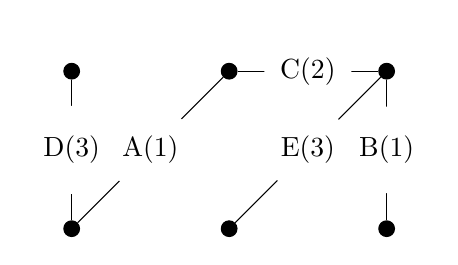
\begin{tikzpicture}
	\begin{scope}[every node/.style={circle,draw, fill= black, inner sep = 2pt}]
	    	\node (1) at (0,0) {};
		\node (2) at (0,2) {};
	    	\node (3) at (2,2) {};
		\node (4) at (4,2) {};
	    	\node (5) at (4,0) {};
	    	\node (6) at (2,0) {};	
	\end{scope}
	
	\begin{scope}[>={Stealth[black]},
	              every node/.style={fill=white,circle},
	              every edge/.style={draw=black}]
		\path (1) edge node{A(1)} (3);
		\path (3) edge node{C(2)} (4);
		\path (4) edge node{B(1)} (5);
		\path (1) edge node{D(3)} (2);
		\path (4) edge node{E(3)} (6);
	\end{scope}
	\end{tikzpicture}
	\\
	The weight of the spanning tree is $1+1+2+3+3=10$.
	
	% 10 b
	\item Repeat part (a) with Prim's algorithm, starting at the lower middle vertex.\\
	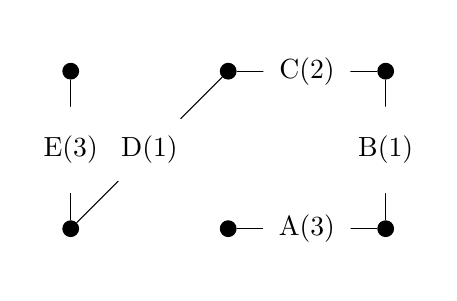
\begin{tikzpicture}
	\begin{scope}[every node/.style={circle,draw, fill= black, inner sep = 2pt}]
	    	\node (1) at (0,0) {};
		\node (2) at (0,2) {};
	    	\node (3) at (2,2) {};
		\node (4) at (4,2) {};
	    	\node (5) at (4,0) {};
	    	\node (6) at (2,0) {};	
	\end{scope}
	
	\begin{scope}[>={Stealth[black]},
	              every node/.style={fill=white,circle},
	              every edge/.style={draw=black}]
		\path (5) edge node{A(3)} (6);
		\path (4) edge node{B(1)} (5);
		\path (3) edge node{C(2)} (4);
		\path (1) edge node{D(1)} (3);
		\path (1) edge node{E(3)} (2);
	\end{scope}
	\end{tikzpicture}
	\\
	The weight of the spanning tree is $1+1+2+3+3=10$.
	\ee

% 11
\item
	\be
	% 11a
	\item Use Kruskal's algorithm to find a minimum spanning tree of the graph below. Label the edges in alphabetical 
	alphabetical order as you choose them. Give the weight of the minimum spanning tree.\\
	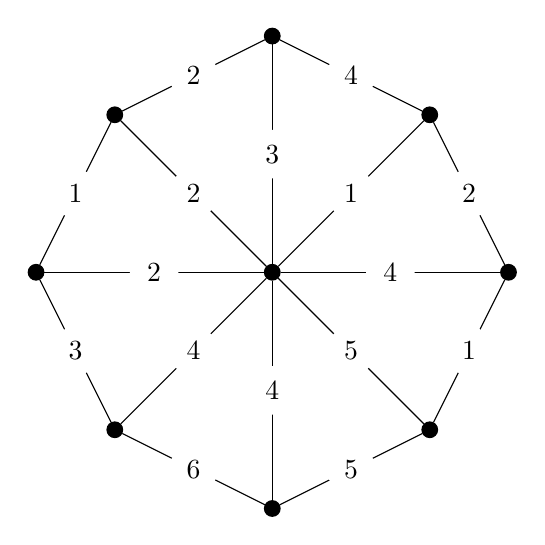
\begin{tikzpicture}
	\begin{scope}[every node/.style={circle,draw, fill= black, inner sep = 2pt}]
	    	\node (1) at (0,0) {};
		\node (2) at (2,-1) {};
	    	\node (3) at (3,-3) {};
		\node (4) at (2,-5) {};
	    	\node (5) at (0,-6) {};
	    	\node (6) at (-2,-5) {};
		\node (7) at (-3,-3) {};
	    	\node (8) at (-2,-1) {};
		\node (9) at (0,-3) {};
	\end{scope}
	
	\begin{scope}[>={Stealth[black]},
	              every node/.style={fill=white,circle},
	              every edge/.style={draw=black}]
		\path (9) edge node{3} (1);
		\path (9) edge node{1} (2);
		\path (9) edge node{4} (3);
		\path (9) edge node{5} (4);
		\path (9) edge node{4} (5);
		\path (9) edge node{4} (6);
		\path (9) edge node{2} (7);
		\path (9) edge node{2} (8);
		\path (1) edge node{4} (2);
		\path (2) edge node{2} (3);
		\path (3) edge node{1} (4);
		\path (4) edge node{5} (5);
		\path (5) edge node{6} (6);
		\path (6) edge node{3} (7);
		\path (7) edge node{1} (8);
		\path (8) edge node{2} (1);
	\end{scope}
	\end{tikzpicture}
	
	% Answer to 11a
	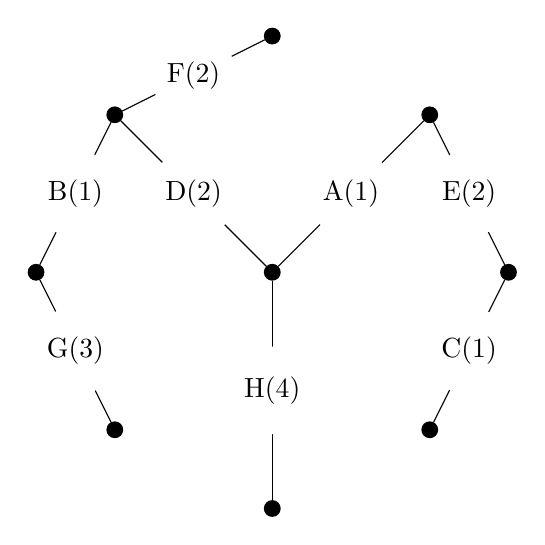
\begin{tikzpicture}
	\begin{scope}[every node/.style={circle,draw, fill= black, inner sep = 2pt}]
	    	\node (1) at (0,0) {};
		\node (2) at (2,-1) {};
	    	\node (3) at (3,-3) {};
		\node (4) at (2,-5) {};
	    	\node (5) at (0,-6) {};
	    	\node (6) at (-2,-5) {};
		\node (7) at (-3,-3) {};
	    	\node (8) at (-2,-1) {};
		\node (9) at (0,-3) {};
	\end{scope}
	\\
	\begin{scope}[>={Stealth[black]},
	              every node/.style={fill=white,circle},
	              every edge/.style={draw=black}]
		\path (9) edge node{A(1)} (2);
		\path (7) edge node{B(1)} (8);
		\path (3) edge node{C(1)} (4);
		\path (9) edge node{D(2)} (8);
		\path (2) edge node{E(2)} (3);
		\path (8) edge node{F(2)} (1);
		\path (6) edge node{G(3)} (7);
		\path (9) edge node{H(4)} (5);
	\end{scope}
	\end{tikzpicture}
	\\
	The weight of the spanning tree is $1+1+1+2+2+2+3+4=16$.
	% 11b
	\item Repeat part (a) with Prim's algorithm, starting at the top vertex.\\
	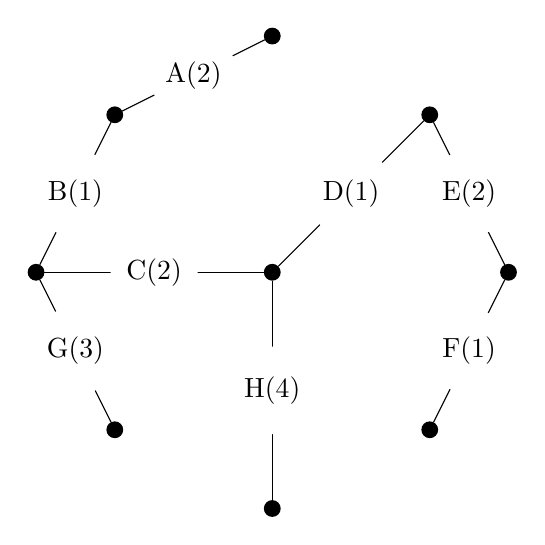
\begin{tikzpicture}
	\begin{scope}[every node/.style={circle,draw, fill= black, inner sep = 2pt}]
	    	\node (1) at (0,0) {};
		\node (2) at (2,-1) {};
	    	\node (3) at (3,-3) {};
		\node (4) at (2,-5) {};
	    	\node (5) at (0,-6) {};
	    	\node (6) at (-2,-5) {};
		\node (7) at (-3,-3) {};
	    	\node (8) at (-2,-1) {};
		\node (9) at (0,-3) {};
	\end{scope}
	\\
	\begin{scope}[>={Stealth[black]},
	              every node/.style={fill=white,circle},
	              every edge/.style={draw=black}]
		\path (1) edge node{A(2)} (8);
		\path (7) edge node{B(1)} (8);
		\path (9) edge node{C(2)} (7);
		\path (9) edge node{D(1)} (2);
		\path (2) edge node{E(2)} (3);
		\path (3) edge node{F(1)} (4);
		\path (6) edge node{G(3)} (7);
		\path (9) edge node{H(4)} (5);
	\end{scope}
	\end{tikzpicture}
	\\
	The weight of the spanning tree is $2+1+2+1+2+1+3+4=16$.
	\ee

% 13
\seti{12}
\item An oil company wants to connect the cities in the mileage chart below by pipelines going directly between cities. What is the minimum number of miles of pipeline needed?
\begin{tabular}{c|c|c|c|c|c|c}
	& Des Moines & Milwaukee & Minneapolis & Omaha & Pierre & Winnipeg\\
	Bismark & 670 & 758 & 427 & 581 & 211 & 369 \\
	Des Moines &  & 361 & 252 & 132 & 492 & 680 \\
	Milwaukee &  &  & 332 & 493 & 690 & 759 \\
	Minneapolis &  &  &  & 357 & 394 & 431 \\
	Omaha &  &  &  &  & 391 & 650 \\
	Pierre &  &  &  &  &  & 521 \\
\end{tabular}
	\\ \\ \\
	Note: Center vertex is Bismark.
	\\
	% Answer to 13
	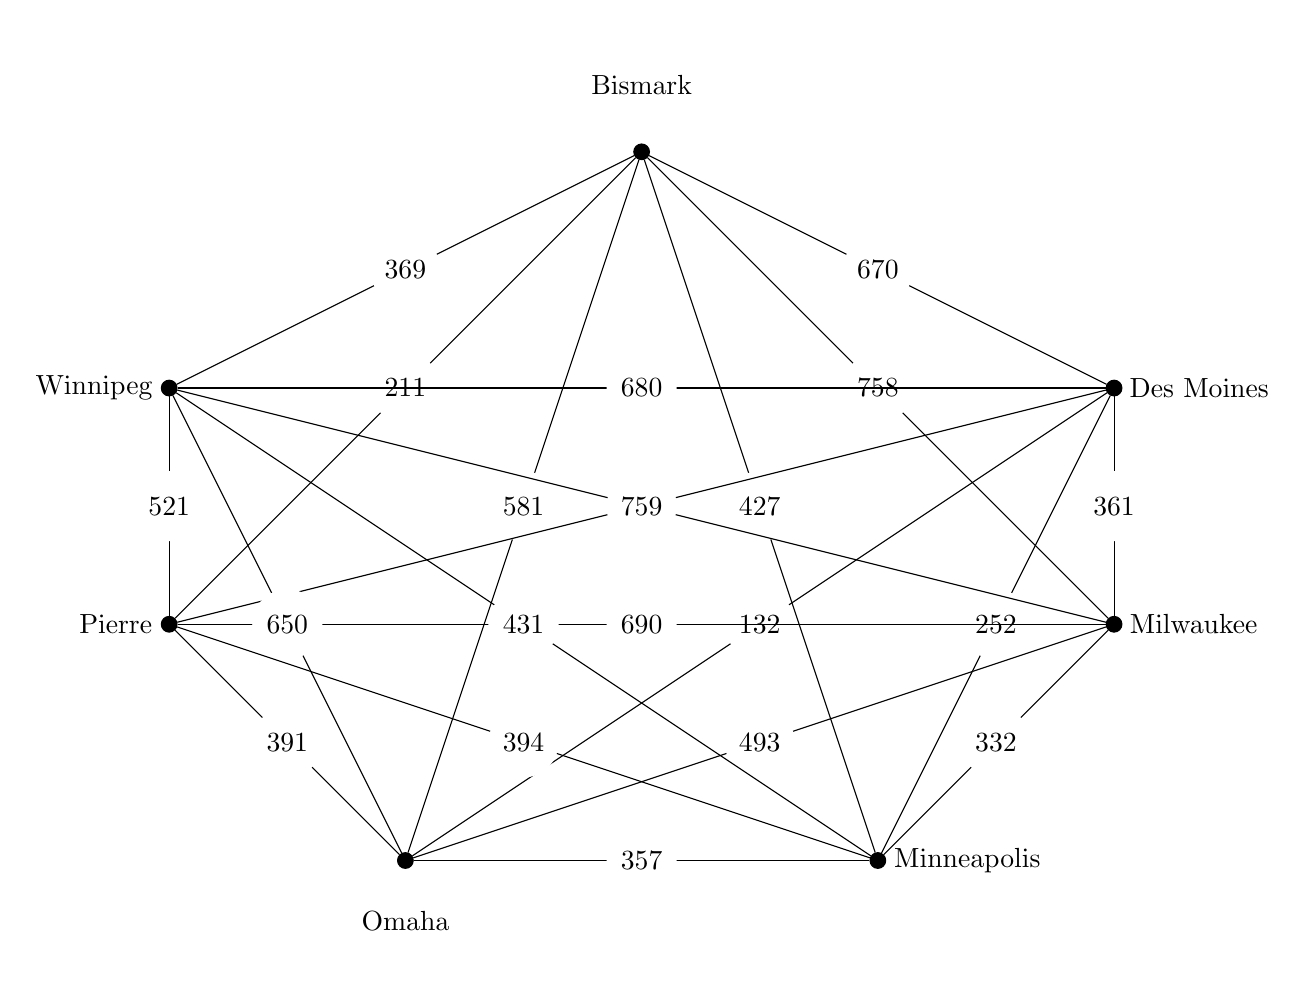
\begin{tikzpicture}
	\begin{scope}[every node/.style={circle,draw, fill= black, inner sep = 2pt}]
	    	\node[label = above:Bismark]		(1) at (0,0) {};
	    	\node[label = right:Des Moines] 	(2) at (6,-3) {};
	    	\node[label = right:Milwaukee] 		(3) at (6,-6) {};
	    	\node[label = right:Minneapolis] 	(4) at (3,-9) {};
	    	\node[label = below:Omaha] 			(5) at (-3,-9) {};
	    	\node[label = left:Pierre] 			(6) at (-6,-6) {};
	    	\node[label = left:Winnipeg] 		(7) at (-6,-3) {};
	\end{scope}
	\begin{scope}[>={Stealth[black]},
	              every node/.style={fill=white,circle},
	              every edge/.style={draw=black}]
		\path (1) edge node{670} (2);
		\path (1) edge node{758} (3);
		\path (1) edge node{427} (4);
		\path (1) edge node{581} (5);
		\path (1) edge node{211} (6);
		\path (1) edge node{369} (7);
		\path (2) edge node{361} (3);
		\path (2) edge node{252} (4);
		\path (2) edge node{132} (5);
		\path (2) edge node{492} (6);
		\path (2) edge node{680} (7);
		\path (3) edge node{332} (4);
		\path (3) edge node{493} (5);
		\path (3) edge node{690} (6);
		\path (3) edge node{759} (7);
		\path (4) edge node{357} (5);
		\path (4) edge node{394} (6);
		\path (4) edge node{431} (7);
		\path (5) edge node{391} (6);
		\path (5) edge node{650} (7);
		\path (6) edge node{521} (7);
	\end{scope}
	\end{tikzpicture}

	\begin{tikzpicture}
	\begin{scope}[every node/.style={circle,draw, fill= black, inner sep = 2pt}]
	    	\node[label = above:Bismark]		(1) at (0,0) {};
	    	\node[label = right:Des Moines] 	(2) at (4,-2) {};
	    	\node[label = right:Milwaukee] 		(3) at (4,-4) {};
	    	\node[label = right:Minneapolis] 	(4) at (2,-6) {};
	    	\node[label = below:Omaha] 			(5) at (-2,-6) {};
	    	\node[label = left:Pierre] 			(6) at (-4,-4) {};
	    	\node[label = left:Winnipeg] 		(7) at (-4,-2) {};
	\end{scope}
	\begin{scope}[>={Stealth[black]},
	              every node/.style={fill=white,circle},
	              every edge/.style={draw=black}]
		\path (2) edge node{132} (5);
		\path (1) edge node{211} (6);
		\path (2) edge node{252} (4);
		\path (3) edge node{332} (4);
		\path (1) edge node{369} (7);
		\path (5) edge node{391} (6);
	\end{scope}
	\end{tikzpicture}
	\\
	The minimum number of miles of pipe needed would be \\
	$132+211+252+332+369+391=1687$ miles.
\ee

\end{document}















